% % % OVERORDNET
% Begreb
% Metode
% Metrik
% Hypotese

% % % ARTIKEL (Mood -> Sociability)
% Hypotese: Positivt humør fører til sociale aktiviteter
% Tidligere: sociale aktiviteter -> affekt
% Metode: Inducering af humør, vurdering af humør, vurdering af fundne aktiviteter

\chapter{Relevant forskning}
Ved at undersøge den nuværende forskning, vil vi først og fremmest fastslå at der er en forbindelse mellem humør og social aktivitet.
Disse vil findes indenfor psykologi-faget.
Vi har en formodning om at måden hvorpå dataindsamling og eksperimentering foregår indenfor dette fag, er ved interview og spørgeskemaer.\bruno{brug kilder som belæg for at det er sådan man eksperimenterer i psykologi}
Dette mener vi at ville kunne gøres bedre med mere objektive data som supplement, som fx. ved løbende forespørgsler via smartphone.
Derfor vil vi til sidst undersøge relevant forskning indenfor dataindsamling på smartphone, specifikt ift. stemningsleje.
Her vil vi også se på allerede eksisterende, indenfor psykologi, spørgeskemaer, for at skabe et grundlag til hvilken slags forespørgsler, samt tidspunkter og frekvens for disse, er relevant.

\section{Sammenhæng mellem humør og social aktivitet}
Ud fra de definitioner der er givet i forrige afsnit, er det humør som vi er interesseret i, da det dækker over længerevarende ændringer, hvilket er tilfældet ved mani-depressive perioder.

For at undersøge den psykologiske forskning og eksperimentering der er foregået op til nu, i forhold til sammenhæng mellem humør og social aktivitet, tages der udgangspunkt i \citet{whelan}.

Det fastslås at der er meget forskning der dokumenterer en 2-vejs forbindelse mellem affekt og social aktivitet\footnote{Engelsk: \textit{sociability}}.
Dog har der været begrænset med eksperimentering til at fastslå at godt humør eller positiv affekt fører til mere social aktivitet, hvilket er hypotesen for eksperimentet i artiklen.
Ud fra en undersøgelse af lignende artikler i den forskning, her tages fat i artikler fra 1986 til selve artiklens publikation (2012), kritiseres den relaterede forskning.
De kritiserer nogle af disse tidligere artikler for at komme frem med en tvetydig retning, altså at det ikke vides om humør påvirker social aktivitet eller omvendt.
Derudover er der også kritik til de tidligere brugte metoder, som fejler i at skelne mellem behagelige og sociale aktiviteter.
Dvs. at der ikke er en klar skelning med de 4 kombinationer; behagelige sociale, ubehagelige sociale, behagelige ikke-sociale og ubehagelige ikke-sociale situationer.

\paragraph{Selve eksperimentet} er delt op i 3 dele.
Første del består i at fastslå aktiviteter med varierende grad af socialitet og behagelighed.
Dette gøres online ud fra en gruppe af 58 studerende, hvor en liste på 82 aktiviteter vurderes på behagelighed og socialitet på en skala fra 1 til 5.
Dette ender ud i en liste af 28 aktiviteter, med en jævn fordeling af behagelighed.

De 2 næste dele er opbygget på samme måde, hvor henholdsvis 138 og 104 psykologi-studerende først ser et video-klip af positiv, neutral eller negativ natur.
Herefter, for at fastslå det nuværende humør, vurderes en række ord, baseret på PANAS (se \cref{panans}), mellem 1 og 7 for i hvor høj grad de opleves i øjeblikket.
Sidste trin er en evaluering af de 28 tidligere fastslåede aktiviteter; hvor de alle på en skala fra 1 til 7 vurderes hvor meget test-personen har lyst til at udføre aktiviteten i øjeblikket.

Det konkluderes ud fra eksperimentet at positivt humør fører til højere lyst til at udføre mere sociale aktiviteter.
Derudover noteres det også at der var en bemærkelsesværdig tendens for de personer der fik induceret negativt humør, havde en højere lyst til ikke-sociale aktiviteter.

\section{Brug af mobil data-indsamling}
Der er fundet to eksempler på brugen af mobil data-indsamling relateret til detektering af humør-ændringer; \citet{social_sensing} og \citet{social_sensing_2}.

\subsection{Social Sensing for Epidemiological Behaviour Change}
% Metode: knytning mellem spørgeskema og ren mobil logning
% Knytter kun de to for 48 timers vinduer, ikke ændring over tid
% For tæt knyttet på fysisk sygdom, så resultater ikke de bedste for psykisk (kun 2 daglige meget store spørgsmål)
I \citet{social_sensing} bruges smart phone data til at undersøge mulighederne for at bruge mobil dataindsamling til at detektere adfærdsændringer, hvilket kan sige noget om en person er syg (fysisk eller psykisk).
Social data indsamles via opkaldshistorik, SMS-historik og bluetooth proximity (hvor muligt) bruges til ansigt-til-ansigt interaktion, samt WLAN-baseret lokations estimering.
Derudover blev der hver dag udfyldt et spørgeskema, bestående af seks spørgsmål angående fysisk og psykisk helbred.

Forsøget blev udført med 70 beboere på et afsnit af et kollegium for bachelor-studerende, hvor de 70 beboere var ca. 80 \% af det totale antal beboere i afsnittet.
Data blev indsamlet fra 1. februar til 15. april (2.5 måned), hvor mobil data blev uploadet døgnet rundt og spørgeskemaer udfyldt hver morgen kl. 6.
Perioden blev delt op i 48 timers intervaller, hvor de spørgeskemaer der blev indsamlet i hvert interval blev knyttet til den indsamlet data for samme interval.

Resultaterne er i mindre grad interessante, da de er nærmere relateret fysisk sygdom og mildere depressioner.
Dog er værd at bemærke at der blev fundet en sammenhæng mellem antallet af opdagede bluetooth devices, wifi rfids, sociale interaktioner og fysisk/psykisk sygdom.
Her er antagelsen at et færre antal devices er resultat af mindre omkring færden.
De personer der meldte sad/lonely/depressed eller havde færre totale interaktioner for samme interval, færre bluetooth og wifi enheder opdaget.
De personer der meldte stress havde ligeså et fald i samtlige mobile målinger, desuden faldt antallet af unikke sociale interaktioner.

\paragraph{Kritik af metode}
Der bruges et meget simpelt spørgeskema, med seks spørgsmål (oversat):
\begin{enumerate}
\item Har du ondt i halsen eller hoste?
\item Løber din næste, er den stoppet eller nyser du?
\item Har du feber?
\item Har du kastet op, har kvalme eller diarré?
\item Har du følt dig ked af det, ensom eller deprimeret på det seneste?
\item Har du følt dig stresset på det seneste?
\end{enumerate}

De spørgsmål der er relateret til psykisk helbred er meget overordnet, og giver derfor kun et groft billede.

Spørgeskemaet blev udsendt hver morgen kl. 6, og på trods af at deltagerne blev betalt \$ 1 for hvert udfyldt spørgeskema blev kun 63 \% udfyldt.
Ifølge \citet{panas} i forsøg udført med henholdsvis 80 og 123 personer, oplevede de mindre affekt om morgenen, hvor den steg hen over dagen, og faldt igen om aftenen.
Dette indikerer at forespørgsel-tidspunkt skal tages med i beregningerne, eller at de skal foretages på flere og mere varierede tidspunkter.

\subsection{Using Social Sensing to Understand the Links Between Sleep, Mood, and Sociability}
I \citet{social_sensing_2} bruges lige så smartphone til indsamling af data.
Her bruges dog kun bluetooth proximity til at tælle antal sociale interaktioner.
Det vil sige at der kun tælles hver gang en forsøgsperson kom i nærheden af en anden forsøgsperson med forsøgets applikation installeret.
Til indsamling af øvrig data bruges daglige, ugentlige og månedlige spørgeskemaer omkring forhold, social aktivitet, humør, kost, motion og søvn.
Disse blev udfyldt gennem smartphone eller web-applikation.

Eksperimentet blev udført med 54 deltager, over en periode på 7 måneder, hvor alle deltagere boede i et samfund med 400 beboere, hvor alle bopæle havde knytning til universitetet.

De 3 undersøgte faktorer; søvn, humør og social aktivitet blev alle simplificeret.
Søvn blev reduceret til 7-værdi skala; 5, 6, 7, 8, 9, samt 2 værdier henholdsvis under og over skalaen.
Humør blev reduceret til en binær værdi; hvor en person for en given dag enten ville være i godt eller dårligt humør.
Social aktivitet blev delt i 2; daglig relativ aktivitet i forhold til den dagen med højest social aktivitet, samt en aggregeret social aktivitet for hver måned.

Ud fra denne data var der 2 interessante resultater.
For det første viste det sig at søvn-længden havde en stor effekt på dagens humør.
For det andet, og måske mere overraskende, viste det sig at jo højere antal sociale interaktioner over en dag, jo bedre sov personen om natten.
Derimod var der ingen mærkbar forskel på antallet af sociale interaktioner for en dag med lav søvn-længde (pånær 5 timer som viser omkring 20 \% færre daglige sociale interaktioner sammenlignet med længere søvn).

\paragraph{Kritik af metode}
Det største problem med den overordnede metode til indsamling af data, er i forhold til indsamling af data vedr. social aktivitet.
Ansigt-til-ansigt interaktion er kun én del ud af den totale mængde sociale interaktion, og derudover var den kun detekterbar mellem de personer der besad smartphone med dertilhørende bluetooth primity app.
Derfor kunne det være at dage med lavere social aktivitet kunne være nærmere knyttet til en mindre lyst til at begive sig udenfor, fremfor lyst til social aktivitet, som så måske kunne detekteres på anden vis.
Et eksempel på social aktivitet der ikke kan detekteres af denne metode er fx interaktion over social medier.

Et andet problem med denne metode er også at kvaliteten af søvn og humør data er lav, så ud over en overfladisk forbindelse kan der ikke siges om hvordan humør og social aktivitet forholder sig i løbet af dagen.
Det nævnes kun kort at personer der generelt havde færre aggregeret sociale interaktioner, generelt havde dårligere humør, hvilket er statistisk signifikant.
Der var også mulighed for at undersøge socialt netværk og ændringen i dette, men er umiddelbart ikke en del af eksperimentet.

\section{Måling af stemningsleje}\label{maaling_af_stemningsleje}
For at kunne indsamle forstyrrende data om en patient er det nødvendigt at vide hvordan dette på nuværende tidspunkt gøres i psykologien.
Derfor er det blevet undersøgt i kilder fra psykologien samt de i fællesrapporten foretagne interviews, hvordan de diagnosticere og evaluerer patienter. 
Disse metoder vil i dette afsnit blive præsenteret.

\subsection{Positive Affect and Negative Affect Scales (PANAS)}
PANAS er en anerkendt liste af begreber relateret til positiv og negativ affekt, som bruges til at vurdere stemningsleje, som beskrevet i \citet{panas}.

% Baseret på tidligere skalaer, bevist uafhængighed begreberne mellem
% Afprøvet præcision med forskellige tidsintervaller
% Afprøvet præcision vha. test/gentest
% Afprøvet som måling af angst, depression og generelt psykologisk lidelse; God correlation ift. NA og kendte skalaer (dårlig, som forventet, correlation mellem PA og samme skalaer)

PANAS er et forsøg på at lave et skema, med skalaer til positiv og negativ affekt, til brug i forbindelse med estimering af humør.
Den er baseret på tidligere eksisterende skalaer, med et ønske om at lave en mere generel og pålidelig skala.
Dette er gjort ved at udvælge og afprøve en række begreber, hvis pålidelighed, præcision og uafhængighed er sikret gennem en lang række analyser og forsøg.

PANAS skemaet er 2 lister af henholdsvis 10 positive og 10 negative ord (oversat):\\
\begin{center}
\begin{tabular}{r | l}
interesseret & irritabel \\\newline
aktiv & fjendtlig \\\newline
eksalteret & skamfuld \\\newline
inspireret & oprevet \\\newline
stærk & nervøs \\\newline
målbevidst & skyldig \\\newline
opmærksom & bange \\\newline
agtpågivende & anspændt \\\newline
entusiastisk & nødstedt \\\newline
stolt & ræd
\end{tabular}
\end{center}
\bruno{Indsæt original fra artiklen i appendiks.}

Alle tyve vurderes med en værdi fra et til fem som indikerer i hvor høj grad begrebet er oplevet.
Om hvorvidt det er oplevet skal tænkes i forhold til en bestemt tidsperiode; \textit{I øjeblikket, I dag, De seneste par dage, De seneste par uger, Det seneste år, Generelt}.

Præcisionen af skalaerne er afprøvet først og fremmest ved at udfylde skemaet med blik på forskellige tidsperioder nævnt ovenover.
Yderligere for at verificere præcisionen, er skemaet afprøvet med samme person, samme tidsperiode(r) flere gange over en periode på femten uger, hvorefter de besvarelserne sammenlignes med en forventning om jo længere tidsperiode jo bedre sammenhold.

Vigtigst af alt er PANAS også blevet sammenlignet med kendte skemaer der bruges i forbindelse med måling af angst, depression og generel psykisk lidelse.
Her vises god korrelation mellem de skemaer og målene for negative affekt for PANAS.
Og omvendt, som forventet, vises dårlig korrelation mellem skemaerne og målene for positiv affekt.\label{PANAS}

\subsection{Stemningsregistrering}\label{stemningsleje::stemningsregistrering}
Under mødet med Psykolog Janne Rasmussen\cite[Afsnit 1.3, Møde med Psykolog Janne Rasmussen]{faelles} blev der nævnt en metode kaldet stemningsregistrering.
Dette afsnit vil kortfattet beskrive denne metode og dens effekt.

Stemningsregistrering\cite[Appendiks F, Stemningsregistrering]{faelles} hjælper patienten med at reflektere over sin stemningsleje.
Det gør at patienten er mere klar over hvordan han har det.
Stemningsregistrering fungerer som hjælpeværktøj under behandlingen, da det er lettere for behandleren at se hvordan patienten har det vha. stemningsregistreringen og samtidig får patienten selv en bedre forståelse.
Stemningsregistrering fungerer ved at patienten hver dag krydser af i et skema, i det felt der svarer til patientens egen opfattelse af sin stemningsleje.
Dette gør at man kan finde mønstre, fx. at patienten er deprimeret hver søndag.
Dette kan så bruges under samtale med behandleren.
Det eneste krav er at patienten kender sine egne symptomer.

Et eksempel på et skema kan ses på \cref{figure::stemningsregistrerings_skema}.
På skemaet kan patienten udfylde fem punkter:
\begin{itemize}
	\item Stemningsleje
	\item Angst
	\item Antal timers søvn
	\item Medicin
	\item Notater og vægt
\end{itemize}

\begin{figure}
	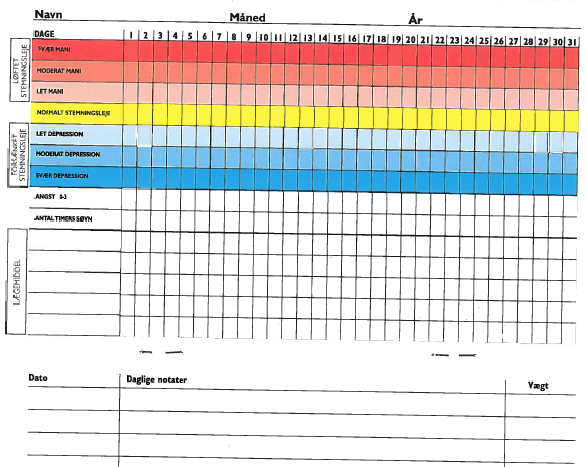
\includegraphics[width=\textwidth]{stemningsregistrerings_skema.png}
	\caption{Et eksempel på et tomt stemningsregistrerings skema.}
	\label{figure::stemningsregistrerings_skema}
\end{figure}

\subsubsection{De fem punkter}
I dette afsnit bliver de fem punkter udspecificeret.
De er baseret på \citet[Appendiks F, Stemningsregistrering]{faelles}.
\paragraph{Stemningsleje}
Under dette punkt er der syv valg:
\begin{itemize}
	\item \textbf{Normal}(gul), hvis der ikke er symptomer på mani eller depression. Energiniveauet er normalt. Søvnen er normal. Forholdsvis nemt at passe daglige aktiviteter.
	\item \textbf{Let mani}(lyserød), hvis patienten føler sig opstemt og optimistisk eller mere irritabel end sædvanligt. Patienten oplever følgende; mere energi, flere ideer, øget selvtillid, mere udadvendt, mere talende, øget sexuallyst, rastløs, sover mindre, vanskeligt ved at arbejde effektivt og fungere socialt.
	\item \textbf{Moderat mani}(mellemrød), griner på upassende tidspunkter eller er meget irritabel og utålmodig, taler meget også selvom andre prøver at sige noget, sover kun fire timer om natten, svært ved at samle sig om en ting, ikke i stand til at passe arbejdet, tænker meget på sex.
	\item \textbf{Svær mani}(rød), ekstatisk, meget grinende eller er vredladen og ofte udskældende, verbale eller fysiske kampe med andre, tror på vedkommende har særlige evner (læse tanker, høre stemmer), konstant bevægelse, sover meget lidt eller ikke, mister kontrollen.
	\item \textbf{Let depression}(lyseblå), lettere trist, selvkritisk, negative tanker, lidt større søvnbehov, svært ved at falde i søvn, træt, er livet værd at leve?, mindre effektiv, kan godt arbejde, andre bemærker det ikke.
	\item \textbf{Moderat depression}(mellemblå), nedtrykt, opgivende, uinteresseret, følger sig langsom, sover mere, svært ved at falde i søvn, bebrejdelse, ukoncentreret, får ikke tingene gjort, selvmordstanker, svært at passe arbejde.
	\item \textbf{Svær depression}(blå), meget nedtrykt, føler intet, håbløshed, energiløs, mistet interessen for alt, ingen appetit, kan ikke sove, alvorlige selvmordstanker, hører stemmer eller ser syner, kan ikke arbejde, svært ved egenomsorg, i sengen det meste af dagen.
\end{itemize}

\paragraph{Angst}
Angst angives på en skala fra og med nul til og med tre.
\begin{itemize}
	\item \textbf{0} svarer til at man ikke oplever nogen form for angst.
	\item \textbf{1} Lettere ængstelig, men påvirker ikke dagligdagen.
	\item \textbf{2} Konstant ængstelig, funktionsniveau påvirkes.
	\item \textbf{3} Udtalt angst, kan næsten ikke foretage sig noget.
\end{itemize}

\paragraph{Antal timers søvn}
Antal timers søvn selvom søvnen har været afbrudt.

\paragraph{Medicin}
Her skrives hvilket og hvor meget medicin der tages i begyndelsen af hver måned.

\paragraph{Notater og vægt} 
Vægten skal registreres mindst en gang om måneden.
Kvinder angiver her de dage de har menstruation.
Andre notater kan være ting som; jobskifte, dødsfald, forelskelse, konflikter osv.

\subsubsection{Information før brug}
Patienten skal oplyses om hvordan han selv finder frem til sit stemningsleje.
Lige nu sker det ved at patienten får udleveret et hæfte som kan ses i \citet[Appendiks F, Stemningsregistrering]{faelles}).
Dette hæfte gennemgås sammen med en psykolog.
Hvis denne metode skal bruges på en mobil platform er det derfor vigtigt at huske at holde dette møde med patienten inden.
Det kan dog også lede op til følgende åbne problemstilling: \textit{Hvordan oplyser vi patienten, om de informationer der er i hæftet, på en mobil platform?}
En mulig løsning kunne være at introducere en gennemgang til første gangs brugere på den mobile platform eller en hjælpe-knap der fortæller om hvert af de fem punkter.

\section{Hamilton Depressionsskala(HAM-D)}
Psykolog Janne Rasmussen fortalte under interviewet at man brugte HAM-D til at afgøre om hvilket depressions stadie man er på.\cite[Afsnit 1.3, Møde med Psykolog Janne Rasmussen]{faelles}
Derfor er HAM-D valgt som en af metoderne til at måle stemningslejet.

HAM-D er en metode oprindeligt udgivet af Max Hamilton \cite{ham_d}, der kan bruges på patienter der tidligere har fået diagnosticeret depression. 
Metoden består af 17 variable faktorer.
Disse variable faktorer giver intervieweren en værdi på 0-4 eller 0-2\footnote{Kommer an på om det er muligt at have et interval på fem eller tre på en given variable faktor.} alt efter hvor meget patienten har symptomet (det maksimale antal point der kan opnås er 52 point).
Intervieweren er en faglig kompetent person indenfor området.
For at gøre det nemmere for intervieweren er de variable faktorer oftest omformuleret til 17 spørgsmål, den danske version kan findes på \citet{ham_d_dansk}.
Når alle værdier er afgivet adderes disse og siger noget om patientens stemningsleje:
\begin{itemize}
	\item \textbf{0-13} ingen depression.
	\item \textbf{13-17} let depression.
	\item \textbf{18-24} moderat depression.
	\item \textbf{25-52} svær depression.
\end{itemize}

Som nævnt foretages HAM-D af en interviewer der er faglig kompetent.
Da spørgsmålene skal præsenteres på en mobil platform lægger det op til følgende åbne problemstilling: \textit{Hvordan præsenteres HAM-D på en mobil platform uden en interviewer?}
En mulighed er at arbejde sammen med en psykolog og en informatiker der sikrer at kommunikere de 17 variable faktorer ud til patienten, så de kan svare på dem.


